\chapter{Laplace and Poisson Equations}
\section{Class notes} 
\includepdf[pages={23-28}]{sources/polyEDP-M1-main.pdf}
\section{Exercises}
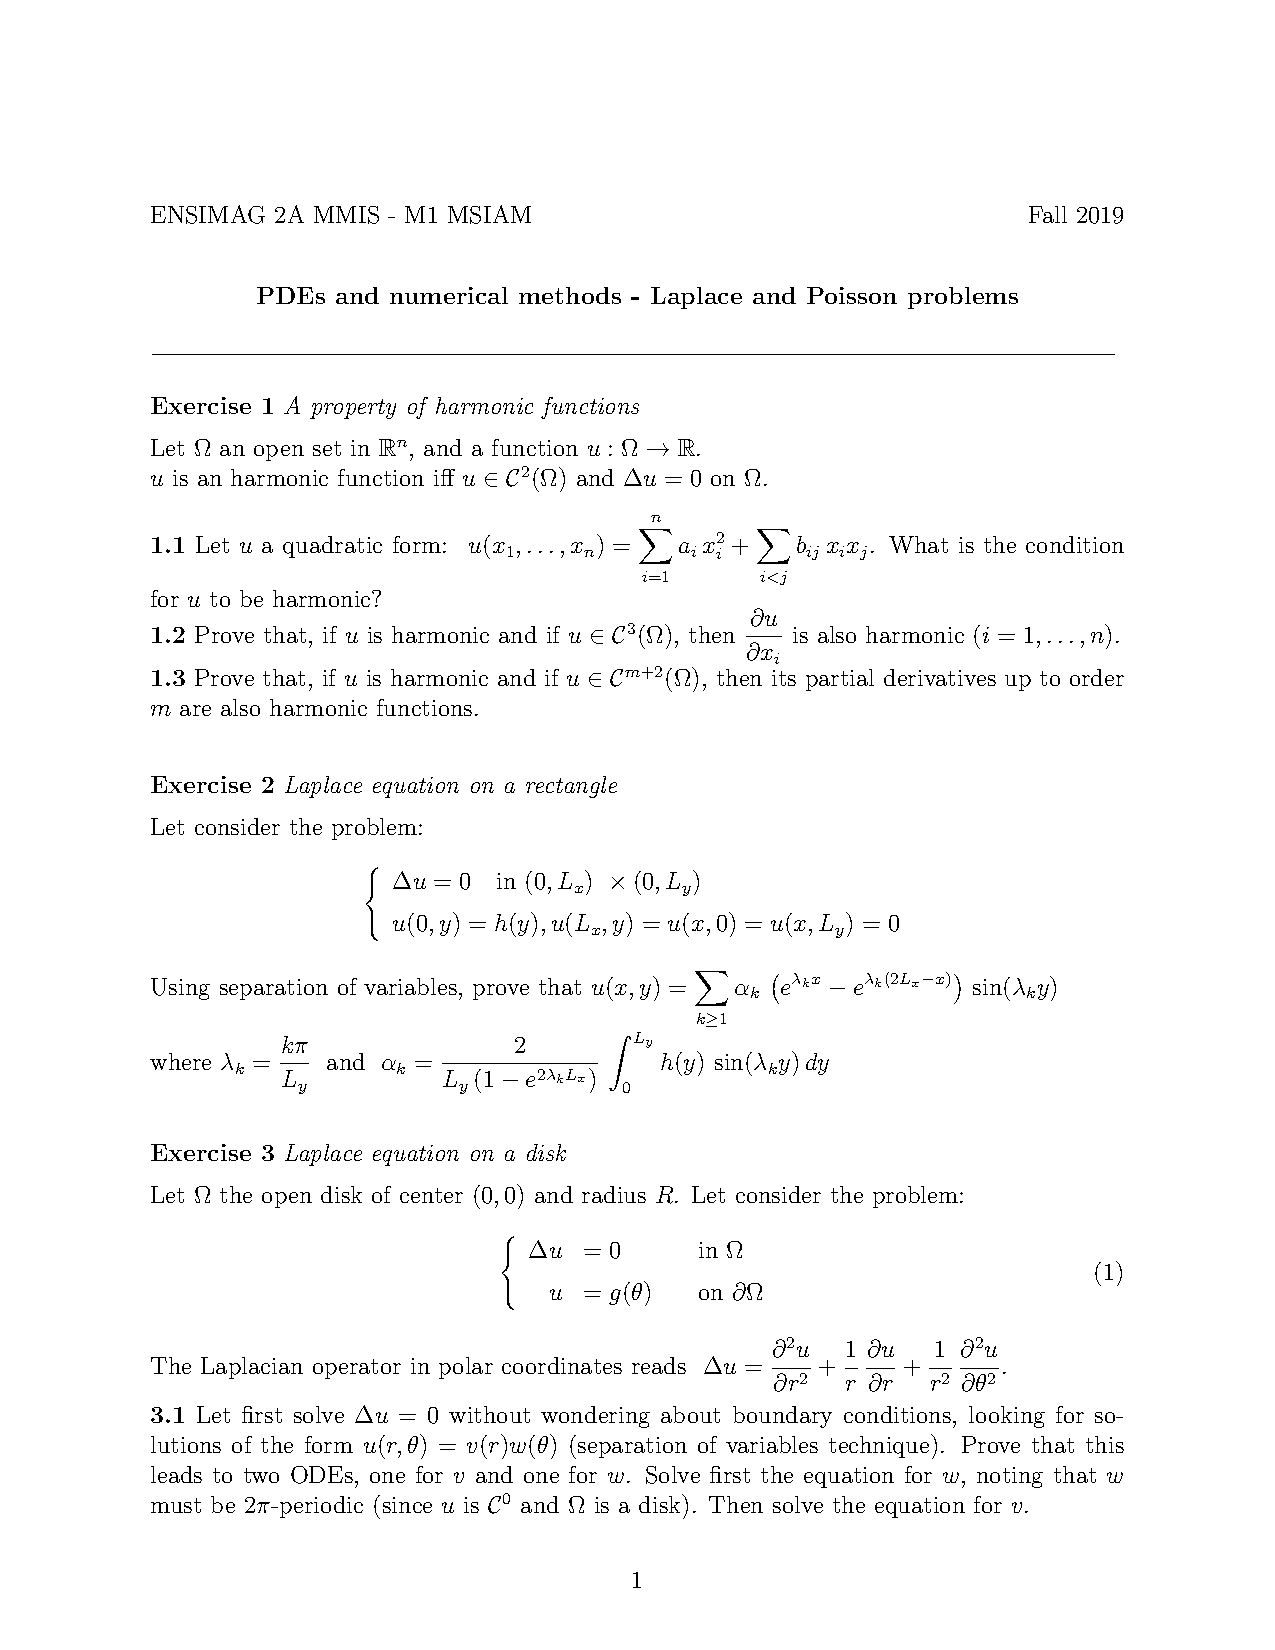
\includepdf[pages=-]{sources/td3.pdf}
\section{Solutions}
\subsubsection{E1 : A property of harmonic functions}
\begin{enumerate}
    \item 
        \begin{align*}
            u  &= \sum_{i=1}^{n} a_i x _{ i }^{ 2 } + \sum_{i<j}^{} b_{ij}x_ix_j \\
            \Delta u  &= \sum_{i=1}^{n} 2a_i + 0 \\
            0  &= \sum_{i=1}^{n} 2a_i  \\
        \end{align*}
    \item 
        Since $ u \in \mathscr{ C } ^3 $, $ \frac{ \partial ^3u }{ \partial x^3_i }  $
        exists 
        \begin{align*}
            \sum_{i=1}^{n} \frac{ \partial ^3u }{ \partial x_i^3 } u &= \sum_{i=1}^{n}
            \left( \frac{ \partial u }{ \partial x_i } \left( \frac{ \partial^2 u }{
            \partial x_i^2 } \right) \right)  \\ 
             & \forall j \in \set{ 1, \cdots, n }  \text{ we have }  \\ 
             &= \frac{ \partial u }{ x_j } \sum_{i=1}^{n} \frac{ \partial ^2 u  }{
             \partial x_i^2  } \\
             &= \frac{ \partial u }{ \partial x_j } \left( \Delta u\right) = 0 
        \end{align*}
    \item Since $ u \in \mathscr{ C } ^{m+2} $, $ \frac{ \partial ^{m+2}u }{ \partial
        x^{m+2}_i }  $
        exists and 
        \begin{align*}
            \sum_{i=1}^{n} \frac{ \partial ^{m+2}u }{ \partial x_i^{m+2} } u &= \sum_{i=1}^{n}
            \left( \frac{ \partial^{m} u }{ \partial x_i^{m+2} } \left( \frac{ \partial^2 u }{
            \partial x_i^2 } \right) \right)  \\ 
             & \forall j \in \set{ 1, \cdots, n }  \text{ we have }  \\ 
             &= \frac{ \partial u^{m} }{ x_j^{m} } \sum_{i=1}^{n} \frac{ \partial ^2 u  }{
             \partial x_i^2  } \\
             &= \frac{ \partial^m u }{ \partial x_j^m } \left( \Delta u\right) = 0 
        \end{align*} 
\end{enumerate}

\subsection{E2 : Laplace equation on a rectangle}
\label{subsec:E2 : Laplace equation on a rectangle}


\subsection{E3 : Laplace equation on a disk}
\label{subsec:E3 : Laplace equation on a disk}


\subsection{E4 : 1D and 2D Laplacian matrices}
\label{subsec:E4 : 1D and 2D Laplacian matrices}


\subsection{E5 : 9-point 2D laplacian - Fourth order scheme }
\label{subsec:E5 : 9-point 2D laplacian - Fourth order scheme }

